\documentclass[../main.tex]{subfiles}
\graphicspath{{\subfix{../../images/}}}
\begin{document}

\chapter{Background \& Prior Work}\label{chap:background}

\begin{quote}
  \emph{Even a simple movement is a global body event.}\\
  \raggedleft{--- Bizzi \& Ajemian, \emph{2020}}
\end{quote}  

\cleardoublepage%

% \begin{quote}
%   \emph{We have some idea as to the intricate design of the puppet and the puppet strings, but we lack insight into the mind of the puppeteer.}
%   \raggedleft{--- Emilio Bizzi \& Ajemian \emph2020}}
% \end{quote}

% (motor maps)
% Ferrier's stimulation studies, idea of motor maps
% evolution leads to more and more CM connections
% connected to a motor field -- group of agonists, interneuron mediated antagonist
% "fractionated control" -- smoothly combining motor activations, glueing together coarser movements -- \cite{heTopographicOrganizationCorticospinal1995}
% string players larger finger map -- Elbert 1995 MEG imaging \cite{elbertIncreasedCorticalRepresentation1995}
% p844 -- image of muscle fields
% p412 -- quotes













% what does this point to?
% maybe put this stuff into conclusions for future work?

% Cortical controllers are massively redundant; the contain all available information about the context of an ongoing task, branching to an array of downstream spinal centers as well as converging to individual spinal innervations. 

% Our theory of neural control of the hand is approximately: control is composed of a number of overlapping cortical controllers. 

% - Motor control is distributed throughout the brain\cite{sejnowskiPerspectivesCognitiveNeuroscience1988}.

% These controllers receive input from goal-oriented centers as well as a plethora of ongoing contextual, perceptual information. 

% - From physiology, we can see that the motor system is highly distributed and constructs action based on a variety of state dependence. The theoretical question becomes \emph{when does it make computational sense to construct action by composing control policies rather than selecting or tuning a single policy?} When is policy arbitration computationally advantageous?

% Control is modulated by these inputs, adjusting “online” to disturbances

% Our hypothesis is that subjects will use their vast repertoire of pre-existing control schemes/movements/controllers/patterns/activations until they find a pattern that increases their success, upon which they will “hone” this scheme by refining the discovered movement. 

% This hypothesis predicts an exploratory, or “search”, period of the task, followed by (or overlapping with) an exploitative or “honing” period as subjects settle on a motor solution. 

% policies, habits, bottlenecks, memory
% - Certain movement disorders can be viewed as involving information bottlenecks -- communicating the policy given your current state \cite{gershmanRewardcomplexityTradeoffSchizophrenia2020}
%   - "optimal compression means knowing the state probabilities" having some form of a model -- marginal state distribution (mean state occupancies?) SR row sums?
%   - "the memory demand of policies acts as an information bottleneck in action selection"
%   - "Default policy" as habits \cite{pirayLinearReinforcementLearning2019}

% - We can speculate that practice and expertise as convincing your brain to commit to a more complex policy (or maintain commitment to a current level of complexity).

% Ideas from theory we can keep in mind for our experiment that we can look out for in interpreting our results:
% - Do subjects display model-based or model-free learning, what would distinguish these two possibilities?
% - Are subjects creating new, bespoke ``controllers'' for this task or are they adapting from existing movement repertoire?
% - Cost functions, optimization
% - System identification (control), policy optimization
% - Implicit / Explicit 
% - Slow / Fast learning rates

% "The challenge for researchers is to find the cost functions that subjects are using", and the learning rule use to update their policies.








%  In this section, we support the claim that the motor system's organizing principle is redundancy at all levels, and that this redundancy supplies us with flexibility. This flexibility is illustrated in the CNS's demonstrated hierarchy in both planning and execution of action. 

%  - what can physiology tell us about the movement problem?
%   - can it inform theory to describe motor solutions?
%   - this will inform the shape our models
%   - the constraints of our tasks, questions
  
% - what do we know about brain and motor?
%   - hands, thumbs, forearms anatomy
%   - synergies, cm connections
%     - bizzi
%     - porter & lemon
%     - from muscles to cortex
%     - 
% - loops and controllers
%   - graziano
%   - cerebellum
%   - cortex, hantman
%   - mouse, primate
%   - basal ganglia  

\noindent Humans produce a great variety of movements every day, often without conscious thought, and the variety of this movement repertoire remains elusive to artificial systems. Movements such as bringing a cup of coffee to our lips are generally out of reach for state-of-the-art robotics. This ``motor gap'' between biological and artificial motor systems is due to a lack of \textit{dexterity}. Soviet neuroscientist Nikolai Bernstein defined dexterity as the ability to ``find a motor solution in any situation and in any condition''\cite{Bernstein1967}. The crux of this definition is the flexibility of motoric solutions. This flexibility, or \textit{robustness}\endnote{Kitano defines robustness as ``the maintenance of specific functionalities of the system against perturbations, and it often requires the system to change its mode of operation in a flexible way''. He claims that robustness requires control, alternative mechanisms, modularity and decoupling between high and low level variability.}\cite{kitanoBiologicalRobustness2004}, is the ability to optimize internal parameters in response to external perturbations and adapt to new information to achieve the goals of an ongoing plan. 

Despite a wealth of impressive work, a holistic understanding of the computations underlying the construction of skilled movement remains an incredibly exciting and fruitful direction of research. Our aim is to progress understanding of skilled movement by studying the solutions produced by human subjects to motor tasks in dynamically rich, yet experimentally manipulable, virtual environments. Our goal is to reverse-engineer the ability to acquire and perform novel motor skills. As our task hinges on our understanding of the structures underlying the production of hand movement, we review here the motor architecture controlling of the hand as it relates to our experiments. In particular, we hope to illustrate how, across levels of the motor system, we find redundancy. This redundancy, we argue, provides the movement machine with its remarkable flexibility.





\section{Motor Units to Muscles}\label{motor-units-to-muscles}

Muscles are composed of fibers which contract due to chemical gradients produced at the neuromuscular junction by action potentials emanating from alpha-motoneurons (AMN) in the ventral horn of the spinal cord. The quantum of motor output is the motor unit (MU), defined as a single motoneuron axon and the set of junctions the terminals of its axon branches form with one or more muscle fibers, as shown in \Cref{fig:motor_units}. The innervation ratio of a particular muscle unit is the number of junctions it innervates. The motor unit provides the motor system with \textit{redundancy} at the muscle level: multiple muscle fibers contract due to a single AMN spike, and multiple AMNs may overlap in their innervations. The forces produced by motor units span several orders of magnitude, though most units produce very small forces. Here we find temporal redundancy: in order to produce movements, MUs combine in time to generate a range of forces\cite{fuglevandMechanicalPropertiesNeural2011}. Since the innervation ratios of muscles in the forearm and hand are relatively small compared to more proximal muscles (which contain thousands of MUs), the logarithmic recruitment and redundancy of motor units enables the hand to produce movements with very fine spatiotemporal resolution via this composition of unit activations.

\begin{figure}[!htb]
  \centering
  \includegraphics[width=0.7\textwidth]{background_theory/spinal.png}
  \caption[Illustration of lower motor system]{An illustration depicting descending axons branching into junctions at two muscles. Each motor unit is defined as the lower motor neuron and all of its neuromuscular junctions. From Kandel et al.\cite{kandelPrinciplesNeuralScience2013}}\label{fig:motor_units}
\end{figure}

% In muscles of the arm, the number of MUs and their innervation ratios each range from tens to hundreds per muscle and per motor unit, respectively, decreasing as muscles become more distal. The well-known signal-dependent noise in models of motor output has been found to be higher for hand muscles than for more proximal muscles, likely due to small numbers of motor units compare to larger muscles[harrisSignaldependentNoiseDetermines1998;fuglevandMechanicalPropertiesNeural2011].

Muscle fibers are contained within muscle compartments, and each muscle may have one or more compartments. The fingers of the hand are extended by the extensor digitorum (ED) which contains four compartments, one for each of the tendons the muscle produces. Each tendon connects to the three metaphalangeal joints of each digit. The fingers are flexed by two muscles, the flexor digitorum superficialis (FDS) and the flexor digitorum profundus (FDP). Like the ED, these muscles produce four tendons, one to each finger from each of their four compartments. As such, one must coactivate these agonist and antagonist muscles in order to extend or flex a single finger in isolation\cite{fuglevandMechanicalPropertiesNeural2011}. Adduction and abduction of the fingers is produced by the nineteen intrinsic muscles of the hand, each of which has their origin and insertion points within the hand itself\cite{vanduinenConstraintsControlHuman2011}. The intrinsic muscle tendons form a kind of network around each of the digits. The human hand, thumb, and forearm system contains more than thirty muscles and at least twenty degrees of freedom are theoretically available for actuation. However, due to biomechanical coupling, the effective degrees of freedom is presumably less than twenty.

% These redundancies at the neurophysiological level play a role in ``spillover'', where contractions of one muscle or muscle compartment seem to spill over into neighboring muscles and muscle compartments. This is evident in the difficulty one has in moving single fingers individually. Spillover has been found in experiments studying the ``recruitment thresholds'' (defined below) of motor units acting on other digits during single digit contractions (Kilbreath \& Gandevia, 1994; Butler et al. 2005; van Duinen et al. 2009). In these experiments, motor units were recorded from one (test) compartment of the respective muscles, while subjects were asked to contract the compartment of the other digits up to 50\% of their maximal force. When the subjects contracted these other digits (one by one), motor units of the test compartment were often recruited. The amount of force produced by the other digits at the time of recruitment of the motor unit of the test compartment is termed the recruitment threshold. The general finding for all three muscles was that, the closer the contracting compartment to the test finger, the more motor units were recruited. [...] One has to ask whether this spillover is functional. Is the frequent recruitment of motor units ac ting on the little finger when we extend the thumb part of a fixed pattern of muscle activation, perhaps to balance forces around the wrist? (Duinen \& Gandevia 2011) 

While the anatomy of the hand and forearm presents constraints on movement, the system remains capable of producing an incredible variety of movement patterns\cite{yanUnexpectedComplexityEveryday2020,Basmajian1963}. This structure exists to facilitate the acquisition of new skills and the generalization of existing skills to new contexts, offering clues as to the relevant computations required for dexterous movement. In \Cref{fig:low_variance_PCs}, Yan et al. show how even low-variance principle components of joint kinematics during object grasping and ASL signing display correlational structure and are not merely noise. That is, the production of hand movement is highly task-specific, where individual tasks are linked to bespoke muscle activations patterns.

\begin{figure}[!htb]
\centering
  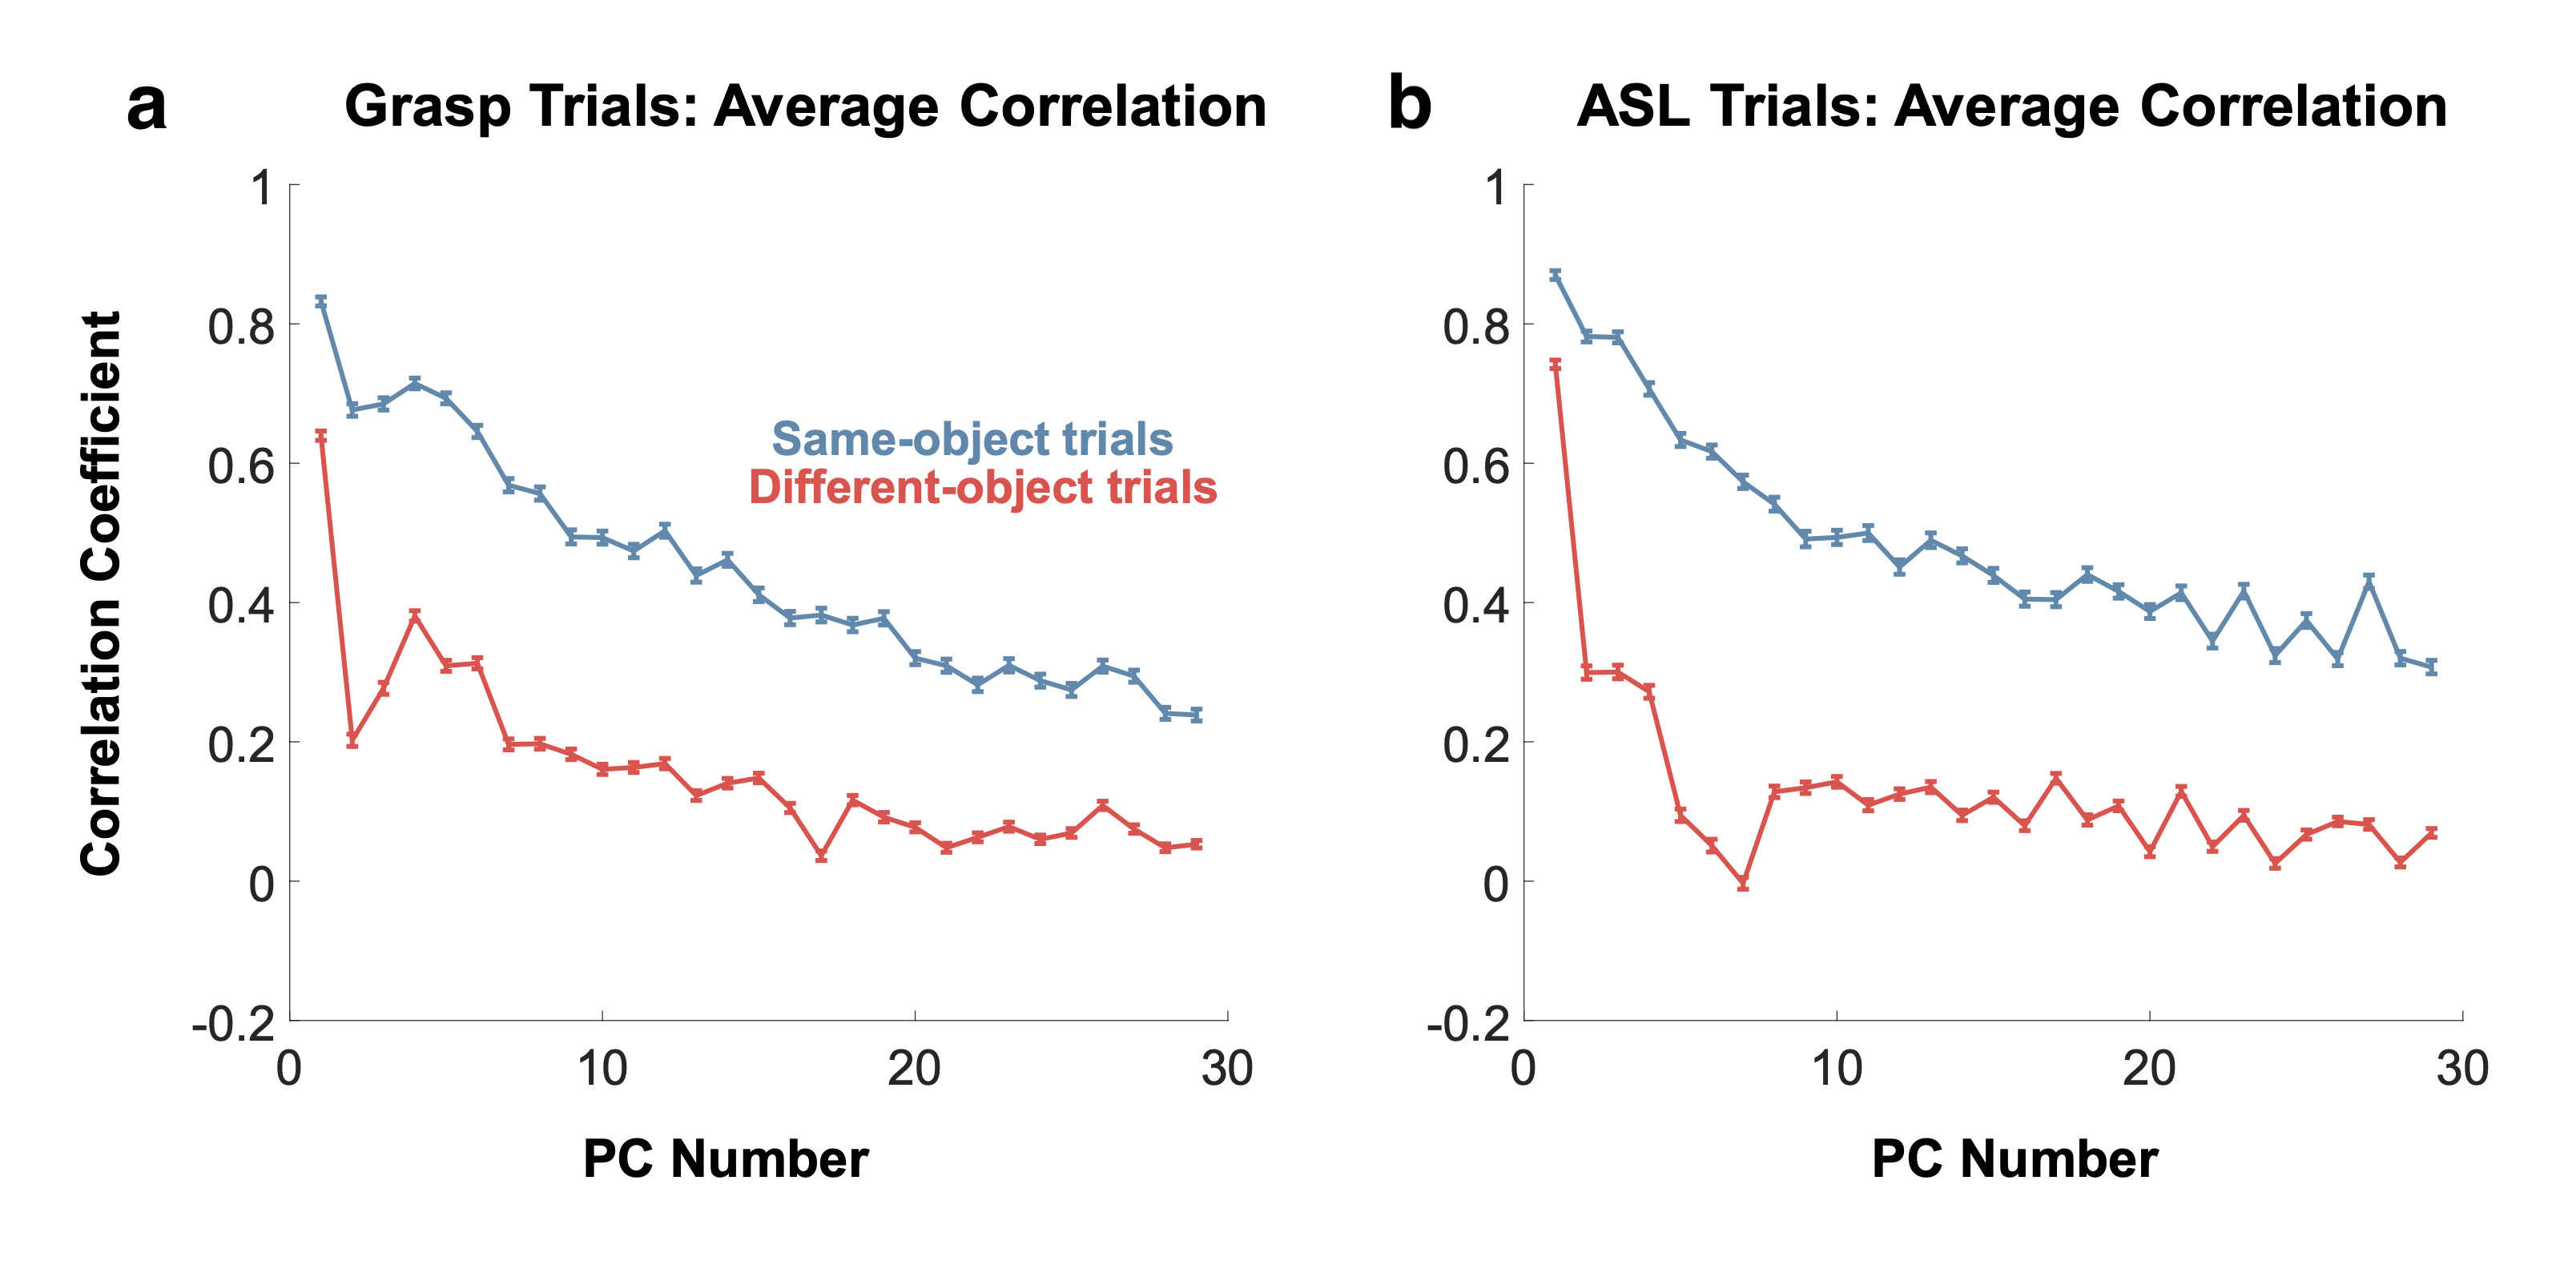
\includegraphics[width=1.0\textwidth]{background_theory/low_variance_PCs.png}
  \caption[Low-variance PCs contain task-relevant information]{Taken from Yan et al.~2020. Plots show mean correlations between hand joint kinematic trajectories during grasp trials with the same (blue) and different (red) objects (a) and ASL signs (b) projected onto the same principle components. Correlations are averaged across 8 subjects. Within-object and within-sign correlations are systematically higher than their shuffled counterparts. Error bars denote SEM. This data supports the idea that low-variance components of kinematics data contain task-specific structure rather than merely reflecting noise. This is encouraging for our experiments, which hope to extend this idea into careful analyses of task specific features of EMG data across learning and in response to perturbations.}\label{fig:low_variance_PCs}
\end{figure}

% \footnote{In a classic study, Basmajian and colleagues showed that it is possible to activate single motor units in the thumb abductor.}

In the 1960s and 70s, there was a surge of interest in this quantum of behavior, the humble motor unit. We take considerable inspiration from work like Basmajian in the 1960s, where basic research was performed on the limits of human motor control, attempting to understand whether humans could learn, with feedback, to fire single motor unit action potentials. We show an illustration of Basmajian's experimental setup in \Cref{fig:basmajian_63}. Variability in performance between subjects varied widely, with some subjects being unable to perform at all, while others able to fire several motor units alone and in concert. In their 1962 experiment, Harrison and Mortenson provide real-time auditory and visual feedback to several subjects attempting SMU activation in the \textit{tibialis anterior} muscle using EMG signals via surface and needle electrodes. They claimed that auditory feedback was more helpful for learning compared to visual feedback and that some form of ``external'' feedback is essential. They report a great variability in response with respect to ability: ``a considerable degree of `mental concentration' is needed for independent contractions''\cite{Harrison1962}. They write that ``As many as six individual motor units were recruited and identified in some experiments'' though this was an extreme level of competency among their subjects. Writing in 1963, Basmajian reports similar findings: ``they groped around in their conscious efforts to find [SMUs] and sometimes, it seemed, only succeeded by accident''. Of those subjects who could do ``tricks'': ``they were unable to explain how they could do it'' though subjects claimed that ``aural feedback was more useful than visual''\cite{Basmajian1963}. Basmajian suggests a mechanism of ``active suppression of neighboring horn cells'' for SMU activation, and calls for ``more exploration of techniques for teaching motor skills''. He writes:
%
\begin{quotation}
\noindent\textit{Although the skills learned in the experiments initially depend on artificial feedbacks, they are learned so quickly and are so exquisite in some persons that they are retained after the feedbacks are eliminated. We do not know the reason because the subjects cannot explain their success or failure, being quite oblivious or of any special feeling. They state that they ``think'' about the previous tests with the cues. This aspect of these studies deserves large-scale investigations for it appears to be of fundamental significance in learning.}
\end{quotation}
%
\begin{figure}[!htb]
  \centering
  \includegraphics[width=0.8\textwidth]{introduction/basmajian_63.png}
  \caption[Basmajian experimental method]{Basmajian's experimental setup, recording single motor unit action potentials from the hands of human subjects.}\label{fig:basmajian_63}
\end{figure}
%
Basmajian conducted a larger follow-up study in 1965 with 54 subjects. 46 could isolate well at least a single unit, while 20 could master a single unit, 18 two, 6 three, and 1 subject four and six units\cite{Basmajian1965}. Subjects found it difficult to ``re-find'' (switch between) and isolate units separately. Wagman, in 1965, suggested that subjects leveraging proprioception to identify SMUs:
%
\begin{quotation}
\noindent\itshape{It appears that without training, volitional activation from the descending pathways is variable. Otherwise, the response of SMUs would not be dependent on maintenance of certain positions of the limb or certain patterns of contractions. During minimal contractions, the action of the descending pathways is modified, and perhaps controlled, probably in the anterior horn of the spinal cord, by peripheral input: proprioception, muscle contraction, or cutaneous stimuli. Therefore appropriate sensory information must be present for volitional activation of SMUs. However, after training, precise conscious control of SMUs can be established with lessened influence of peripheral stimuli.\cite{Wagman1965}}
\end{quotation}
%
Thus, the limits of human motor control, as evidenced by these experiments, extend to the very ends of the motor spectrum. In this work, we take up Basmajian's charge of constructing a large-scale version to continue along the trail blazed by these early, inspirational works.

% Basmajian quotes: 
% ``After individual motor units within the field of a surface or needle electrode were recruited, the subject attempted to isolate and contract the units independently.``
% isometric and isotonic contractions
















\subsection{Coordinative Structures}\label{coordinative-structures}

Many studies have contributed to the concept of synergies as a hard-wired organizing feature of the motor system\cite{mussa-ivaldiMotorLearningCombination2000b,DAvella2003}. However, these works tend to extrapolate from non-primate preparations, particularly in the frog, and use tasks which are inherently low-dimensional to explain covariance structure in primate and human kinematic and electromyography data\cite{giszterMotorPrimitivesNew2015,gaoTheoryMultineuronalDimensionality2017}. That said, it would be foolish to deny the existence of synergistic muscle coactivation even at the structural level. Careful studies of force control by the fingertips present a complex story of dimensionality of control in this regime\cite{raczSpatiotemporalAnalysisReveals2013}. While constraints certainly exist in the architecture of the hand as well as its control system, we maintain that the concept of synergies, especially in the context of dexterous movement, is often presented as an oversimplification rather than a mere simplification. We believe the story of the hand is more complex.

Studies have attempted to quantify the number of effective degrees of freedom of the hand with various methods. This has primarily been taken to be the number of linear features which contain a desired level of the original signal variance, where the signal is the joint angles of the hand engaged in various behaviors\cite{Ingram2009,TodorovDimensionality2005}. These methods have resulted in roughly 8 linear features of hand kinematics to solve a variety of tasks, with subtleties found in inter-task and inter-subject variations. While we accept that the motor repertoire is hardly high-dimensional when compared to the dimensionality of the visual feature extraction system, a recent study found that low-variance linear, kinematic components displayed significantly higher correlation within condition (e.g.~grasp of a specific object) than across conditions. This suggests that these components carry task-dependent information rather than condition-independent, task-irrelevant noise, that the control of the hand is more nuanced than a set of fixed synergies\cite{yanUnexpectedComplexityEveryday2020}.

What Bizzi and colleagues call ``the problem of supraspinal pattern formation'' (how synergies are activated through time) we argue, in the context of hand control, is not \textit{simplified by} the existence of hard-wired or soft-wired synergies\cite{bizziMotorPlanningExecution2020}. Rather, the CNS produces control signals in a range of contexts and in response to continually changing task demands. Rather than the CNS ``simplifying movement'' through synergetic action, it is more likely that hand synergies fall out of a optimization strategy which trades off effort and accuracy where effort may, in part, correspond to independent control of individual control dimensions. In this view, synergies, hard-wired or not, reflect the statistics of the environment in which movement is constructed\cite{brutonSynergiesCoordinationComprehensive2018}.

A considerable amount of discussion has focused on the existence of synergies as a simplifying structure which allows the motor system to ``solve'' the redundancy ``problem''. Synergetic control implies control in the space of a low-dimensional set of synergy weights rather than independent control over the actuator dimensions themselves. The control dimensions are functionally coupled as a result of synergetic action, which both simplifies the control task and constrains behavior to the low-dimensional subspace defined by the synergy weights\cite{merelHierarchicalMotorControl2019}. This is what Bizzi and colleagues refer to as ``the puppet's strings''. The term can also be used as a normative model of motor coordination which implies a constraint in the dimensionality of the descending supraspinal control signal, the simplifying movements of the puppeteer.

In other words, coordination between two or more effectors (muscles, joints, limbs, or even different people) occurs when the motor commands sent to one effector depend (in a causal or statistical sense) on the state of the other effector(s). We argue that coordination is goal-directed; the interdependency of movements is driven by the achievement of a behavioral task. If we limit ourselves to synergetic control as a constraint rather than strategy, we have simply passed the problem to a lower-dimensional one of the same fundamental nature. Neural control of the hand likely contains a spectrum of modularity in order to maintain its role as a flexible instrument. Synergetic action is one end of this spectrum resulting from the computations inherent to, along with the structures of, the human movement machine.


% The term “synergy” is often introduced to explain coordination across different muscles. As a descriptive term, a synergy simply refers to the strong regularities in the spatiotemporal pattern of muscle commands, and the observation that large portions of the variance of recorded muscle activity can be described by a small number of linear components (d'Avella et al. 2006). As an explanatory term, a synergy refers to a neural controller that produces the correlated pattern of muscle activity. 

% In the framework of Optimal Feedback Control, coordination in both feed-forward and feedback control is achieved by making the control policy of one effector dependent on an internal estimate of the state of another effector (Todorov et al. 2002, Diedrichsen et al. 2010). The difference between feed-forward or feedback control within this framework is gradual, and simply reflects the fact that the state estimate is informed by an internal prediction in the former, and actual sensory information in the latter case. 

% Nikolai Bernstein coined the phrase "the degrees-of-freedom problem" to describe the challenge the motor system faces in coordinating its many dimension to achieve a goal. Solving this problem requires dexterity [Bernstein1967]. As we have seen, redundancy is present from joints and muscles to motor units and their upstream synaptic partners. However, rather than asking how the motor control system deals with this "problem" overwhelming complexity, we might instead question why this complexity evolved at all. What does the availability of this redundancy afford the motor system? How does this redundancy enable dexterous movement? 

% The term ``motor synergy'' can be used descriptively to describe the spatiotemporal coactivation of muscles necessary for an ongoing task.  







\subsection{Fractionating Structures}\label{fractionating-structures}

Just as many muscle fibers may be innervated by a single AMN, up to thousands of neurons contact single AMNs through monosynaptic corticospinal, or corticomotoneuronal (CM), connections and other descending pathways through elaborate spinal circuitry. The hallmark of CM connections in particular is their influence over multiple muscle compartments as well as multiple muscles, though typically agonist or antagonist sets\cite{cheneyFunctionalClassesPrimate1980}. This may seem counter-intuitive as a means to produce individuated movement, but experimental evidence in primates has shown that the convergence of many CM collateral fibers onto single AMNs driving the distal muscles in particular can produce a fine grading of activity over motor units driving the distal joints. CM cells also appear to play a role in the inhibition of antagonist muscles prior to contractions required for movement \cite{griffinMotorCortexUses2020}. These findings confirm theories about the excitatory and inhibitory role of these connections dating back decades, and combine to suggest that variables encoded in cortical ensembles are more complex than kinematics or dynamics alone\cite{cheneyFunctionalClassesPrimate1980}.

Years of research have contributed to a complex picture of hand function which embraces non-synergistic movement. The key insight of this body of work is: while ``the organization of the spinal cord is based on relatively rigid muscular modes, a mechanism to fractionate this is of particular importance for the muscles of the hands and digits which may need to be employed in a variety of flexible associations during voluntary movements''\cite{lemonCorticalControlPrimate1993,lemonMechanismsCorticalControl1997,lemonDescendingPathwaysMotor2008}. Careful anatomical work has shown how monosynaptic corticospinal, or corticomotoneuronal (CM), connections provide such fractionation in primates which use tools requiring dexterity.\endnote{CM connections are specific to the primate corticospinal tract and specific to distal muscles of the hands and arm. It appears that the rodent CST contains CM connections until around P10 at which point they recede. Thus, practically CM connections are a feature of primates, though their evolutionary roots are much older\cite{guControlSpeciesdependentCorticomotoneuronal2017,murabeHigherPrimatelikeDirect2018}.}

The CM tract thus acts in coordination with synergistic muscle activations of the hand to achieve control that is balanced between modularity and flexibility. Findings suggest that there is a bipartite structure in human motor cortex driving dexterous control of the distal part of the upper limb which, it has been suggested, evolved under pressure to quickly generalize between tasks. This work argues that these two streams of hand control, namely ``fractionated'' and ``synergistic'' control, may interact to produce versatility, and balancing these subsystems may be a key part of the optimization function when learning new skills\cite{Rathelot2009,griffinCorticomotoneuronalCellsAre2015,Takei2017}. This dualism is likely not rigidly dichotomous, but rather a spectrum of overriding fractionation (so-called ``New M1'') atop a phylogenetically older system of synergistic action\cite{dumCorticospinalSystemStructural2011}. Griffin and colleagues found that CM cells are functionally tuned to a muscle's mode of activity (agonist, antagonist, fixator) to ``bypass spinal cord mechanisms and sculpt novel patterns of motor output that are essential for highly skilled movements''\cite{griffinCorticomotoneuronalCellsAre2015}. 

The degree to which fractionation of movement is, or can be, learned remains unknown. Skilled piano performers have been found to exhibit a higher degree of independent movement among the fingers compared to control participants. Control groups displayed a hierarchical, presumably lower dimensional, organization of finger movement patterns while pianists showed distinct but individuated movement patterns \cite{furuyaFlexibilityMovementOrganization2013}. These results imply that with skilled practice humans can produce finer, more independent movements of the fingers, and construct bespoke coactivations to solve specific goals. Similarly, studies have found that coherence between the index finger and thumb is greater on the dominant hand. This might imply a developmental lateralization, but use-dependent plasticity due to greater precision grip behavior of the dominant hand is also a viable explanation\cite{fuglevandMechanicalPropertiesNeural2011}.

The previously described work suggests a hypothesis: CM connections override the ``consolidated'' patterns putatively generated via spinal interneuron circuitry. The experimental methods devised in our work aim to measure fractionation by tracing motor unit correlations across learning. Whether fractionation in our experiments is due to the CM pathway can only be speculation, but our work may provide direction for future studies pairing intracortical recordings with careful electromyography.



% Individual corticomotoneurons contact multiple motor pools, and rarely (if ever) individual motor neurons. 

% > It is generally believed that the direct corticomotoneuronal (CM) pathway, which is a phylogenetically newer pathway in higher primates, plays a critical role in the fractionation of muscle activity during dexterous hand movements. However, the present study demonstrated that PreM-INs, which are phylogenetically older, have spatiotemporal properties that correlate with muscle synergies during voluntary hand movements. Therefore, it is likely that these two systems have specialized functions for the control of primate hand movements, namely “fractionated control” and “synergistic control,” respectively. The interaction of these two putative control systems might be the source of the exceptional versatility of primate hand movements. [...] Optimization of balanced control may be an important factor also for the acquisition of new motor skills [Takei2017]. 

% The concept of a balanced control may prove to be a fruitful direction for theoretical work on dexterous motor control, the goal being to construct a model which takes into account this spectrum of individuation into account. The experimental challenge is to identify tasks which ostensibly require the direct descending connections to fractionate learned synergies. There is work suggesting that CM connections synapse primarily on low threshold, low force motor units that are recruited first. This would imply a difference in synergy fractionation at lower force as opposed to higher force. This can be tested easily by including a force parameter in a hand control task. The hypothesis stemming from the previously described work is that CM connections override the "consolidated" patterns putatively generated via spinal interneuron circuitry. 

% Recent working studying patients with cerebellar ataxia suggests that the cerebellum plays a role in the temporal recruitment of behavioral syllables, while motor cortex may be implicated in the spatial structure of synergetic action, though this study focused on 13 proximal muscles of the shoulder and arm rather than the distal muscles driving the hand[bergerDoesCerebellumShape2020]. 

% \Cref{fig:strick_graziano} depicts the hierarchical nature of the motor system that enables its dexterity. The motor system is tuned to produce varying levels of modularity, and this is shown in Rathelot's work at a structural level: CM cells evolved to provide modifications to coarse, synergistic action. This is reflected in Graziano's work where, loosely, more dexterous behaviors are produced when stimulation is applied to the caudal regions of motor cortex. These dexterous behaviors are driven by a hierarchical stack of cellular machinery, each level of which is modulated by estimated state, goals, uncertainty, and value. 

% The movement machine reasons in the space of feedback control systems and their ensuing trajectories. The phenomenal thing about the motor system is that it is able to tune itself rapidly with both high-dimensional sensory inputs and sparse reward signals[bahlNeuralDynamicPoliciesfor2020;ijspeertDynamicalMovementPrimitives2013]. This has some precedence in the literature and will be discussed further in {sec:theory}. This section has attempted to illustrate the complexity of the motor control system specifically with regard to dexterous control of the hand, with an eye toward experimental and theoretical avenues for exploration. The goal is to build and test a theoretical scheme for aspects of the compositional nature of the neural hand controller. 







\subsection{Supraspinal Motor Maps}\label{supraspinal-motor-maps}

It is known from recent work that primary motor cortex (M1) is not an isolated movement-generating dynamical system, but rather a node in the network of a feedback-modulated, distributed movement machine\cite{sauerbreiCorticalPatternGeneration2019}. Thinking of the structural architecture of M1 as an input-driven system with outputs along a spectrum of modularity from synergistic to fractionated, we can ask what kind of functional architecture might have evolved in the neuromuscular controller? Graziano and colleagues found that 500ms electrical stimulation to M1 reliably produced stereotyped movements in primates\cite{grazianoOrganizationBehaviorialRepertoire2006}. These movements appeared to produce goal-oriented actions pulled out of other contexts such as bringing food to the mouth, and seemed to be arranged on the cortical sheet topographically in terms of spatial endpoints rather than as a humunculus. Graziano refers to this as the cortical ``action map'', that these stimulations tapped into the control mechanisms of the primate's motor system\cite{grazianoIntelligentMovementMachine2009}. These results has recently been confirmed by optogenetics work in marmosets and macaques \cite{ebinaArmMovementsInduced2019,watanabeForelimbMovementsEvoked2020}.

The motor map concept suggests interpreting activity in M1 as a field of feedback control microcircuits, integrating and transforming inputs, both internal and external, to sculpt ongoing movement\cite{wiltschkoMappingSubSecondStructure2015}. This is in accordance with the idea that there is a structural hierarchy in M1 covering a spectrum of movement modularity. These ideas together form a picture of the motor system as a structural scaffold upon which behaviorally relevant feedback mappings from cortex to the spinal cord are continuously activated and modulated based on information and estimates about the periphery, in line with Basmajian and colleagues' intuitions that proprioception and other sensory feedback plays a key role in modulating motor outputs. In this view, the encoded variables of interest depend on the goals, context, and perturbations of the intended movement. \Cref{fig:strick_graziano} shows Graziano et al.'s stimulation results, what might be termed a \textit{functional view} of the cortical motor system, next Strick et al.'s work described above clarifying the \textit{structural view} of modularity in this system.

\begin{figure}[!htb]
  \centering
  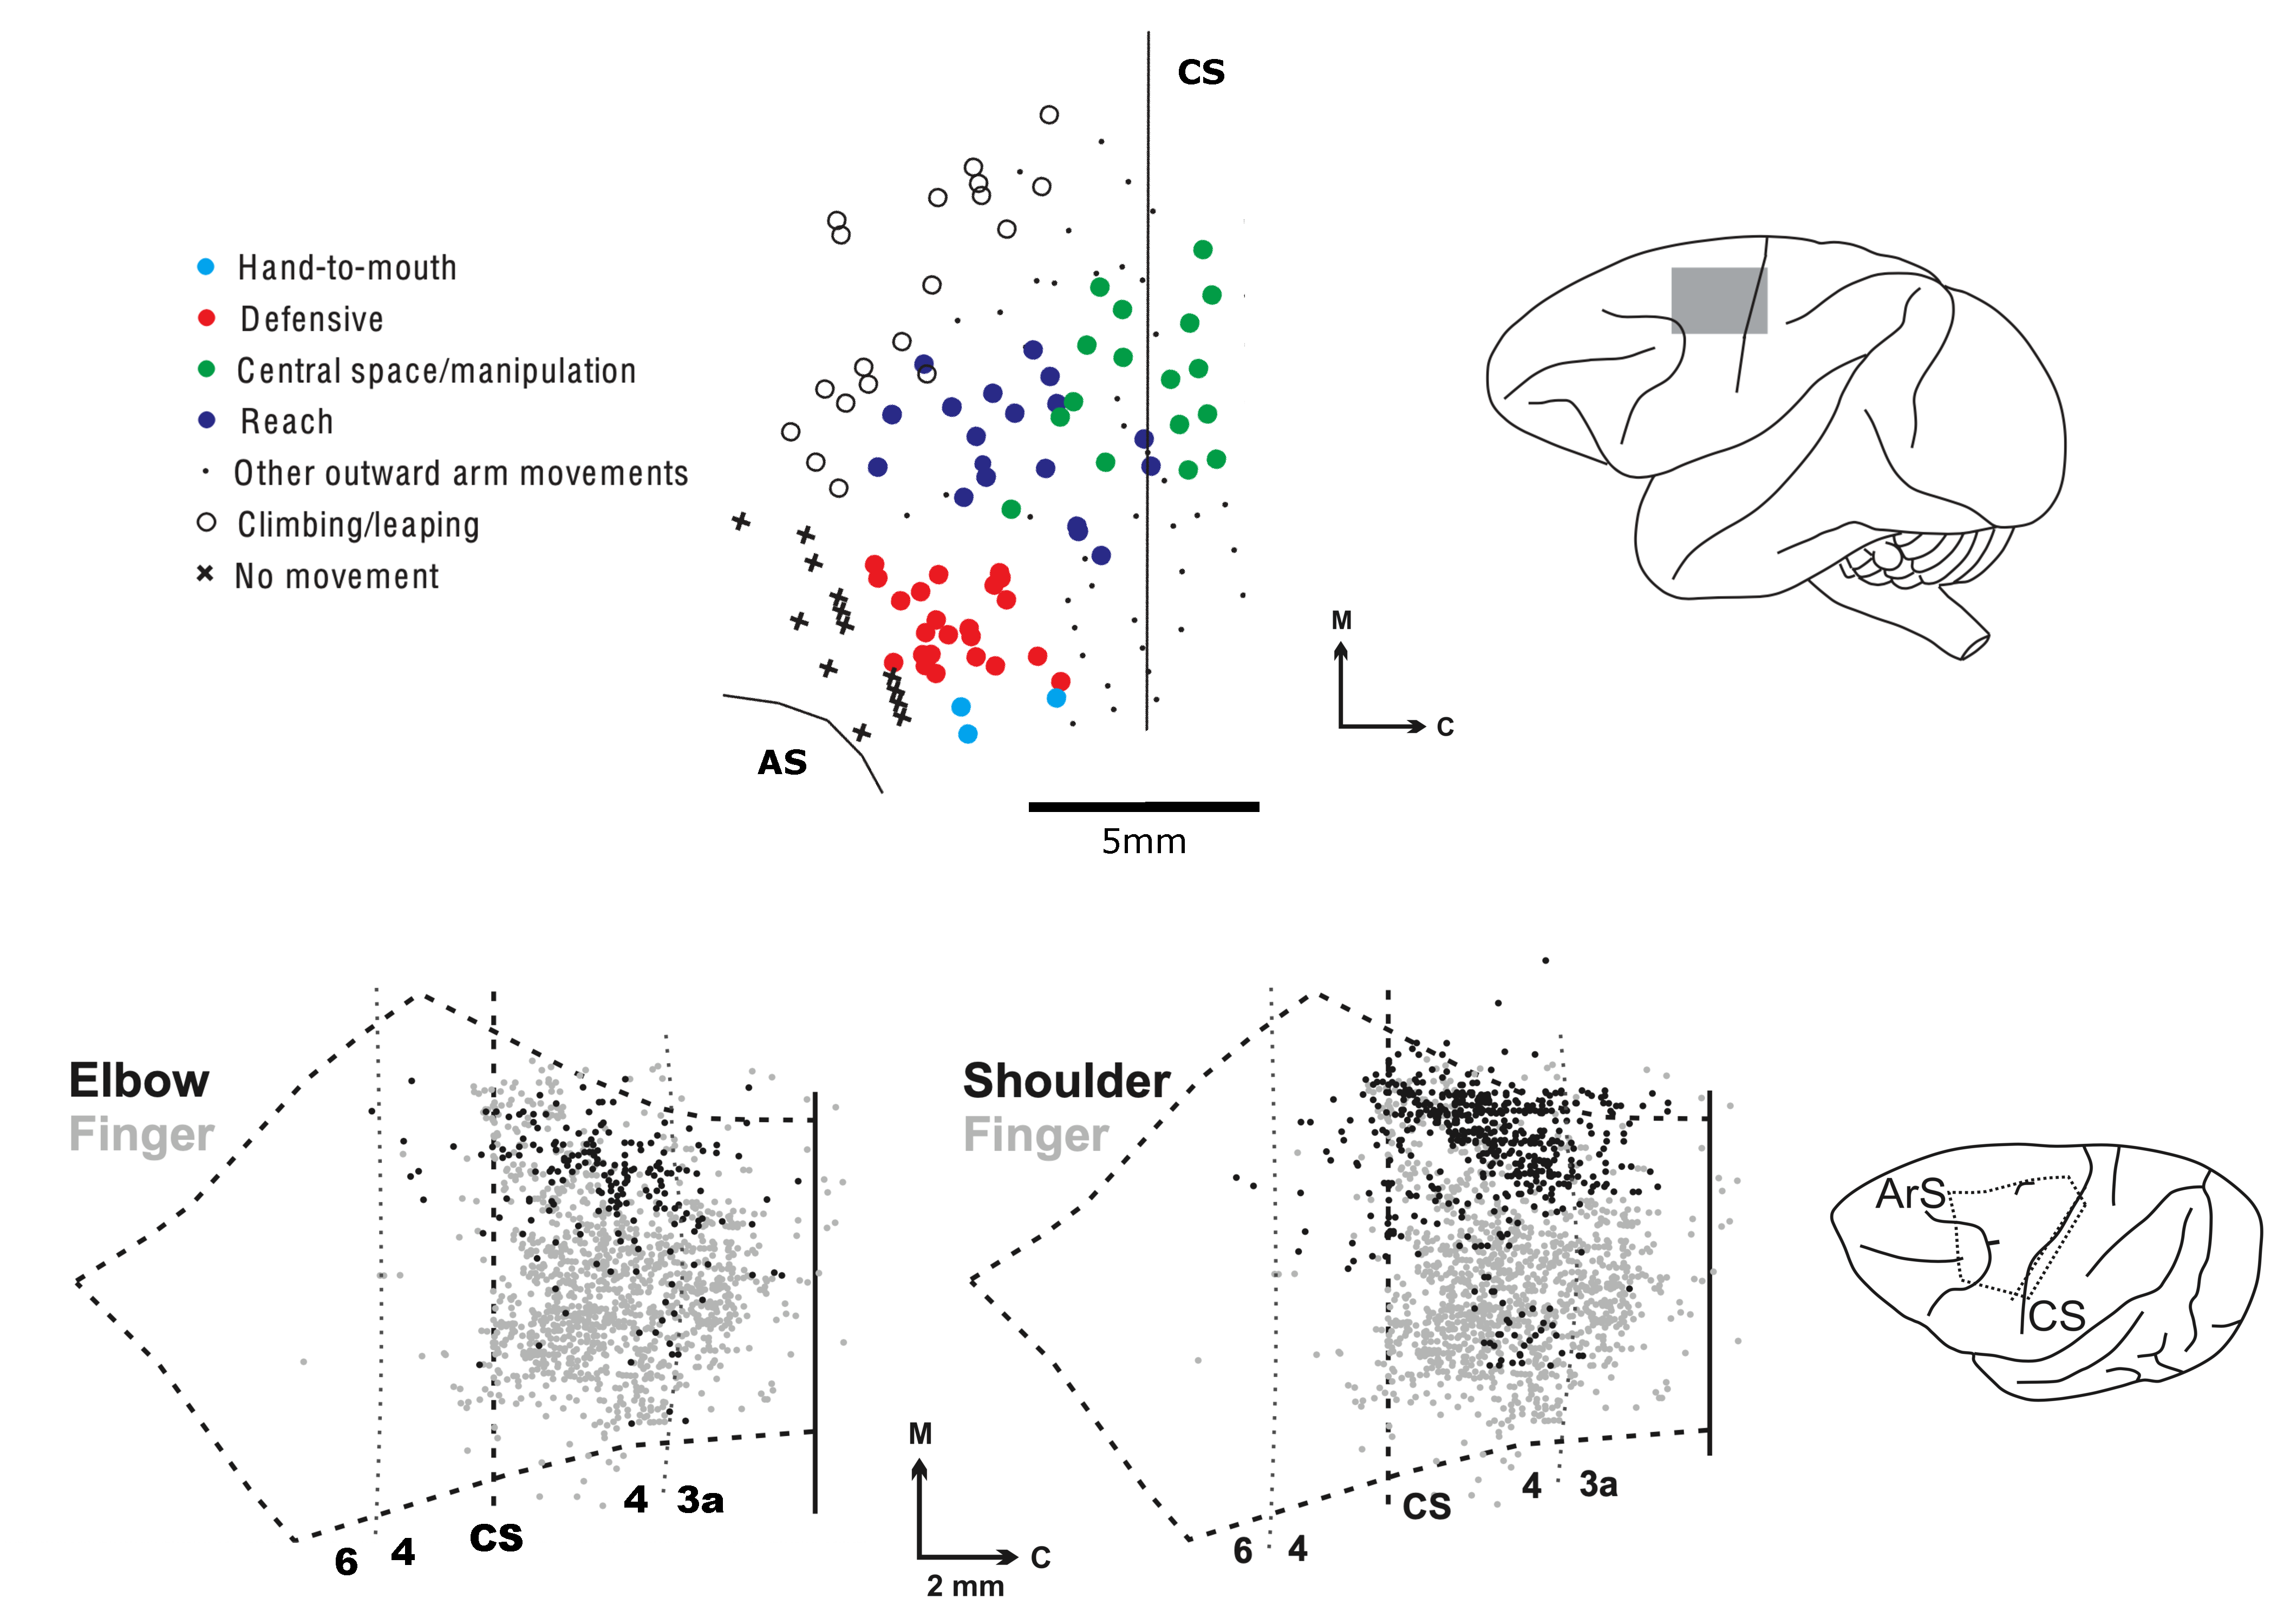
\includegraphics[width=1.0\textwidth]{background_theory/strick_graziano.pdf}
  \caption[Comparing the work of Strick and Graziano]{Similarities between electrical stimulation on behavorial timescales and rabies tracing identification of CM cells. CM cells are largely confined to the caudal half of M1, while this region tends to evoke complex manipulatory movements when electrically stimulated. (Bottom Left) Corticomotoneuronal (CM) cells traced using rabies from muscles of the elbow and finger. (Bottom Right) CM cells traced using rabies from muscles of the shoulder and finger. (Top) Complex movements evoked by 500ms electrical stimulation pulse trains. Adapted from Graziano 2005 and Rathelot et al.~2009\cite{grazianoArmMovementsEvoked2005,Rathelot2009}.}\label{fig:strick_graziano}
\end{figure}

Graziano writes:
%
\begin{quote} 
  The usefulness of a feedback-dependent mapping from cortex to muscles is that it can in principle allow neurons in motor cortex to control a diversity of movement variables, such as direction, speed, hand position, or posture that transcend a fixed pattern of muscle activation. If the network receives feedback information about a specific movement variable, then it can learn to control that variable.
\end{quote}
%
Muscle activity is, in this sense, a readout from a network transforming state-dependent inputs into movement goals. Rather than choosing muscle patterns in reconfigurable blocks, it creatively constructs and sculpts movement. The hierarchy of the motor system may not be rigidly organized around a particular set of variables. As shown in \Cref{fig:motor_system}, many loops exist connecting cortex with the spinal cord, the cerebellum, the basal ganglia, and the sensorimotor periphery. Each of these loops contributes information for the flexible activation of the relevant action maps. Put simply, prevailing evidence suggests that cerebellar loops provide predictive state information while basal gangliar loops provide state and/or action value information. Taken together, this work provides an image of the incredible complexity which generates dexterous movements of the hand. This is the foundation on which we can work to build experiments which elucidate the computations involved in the production of skilled movement. We aim to connect our results back to what is known about the system we are attempting to reverse-engineer in order to inspire future inquiries into the inner workings of the movement machine at both a functional and structural level.

\begin{figure}[!htb]
\centering
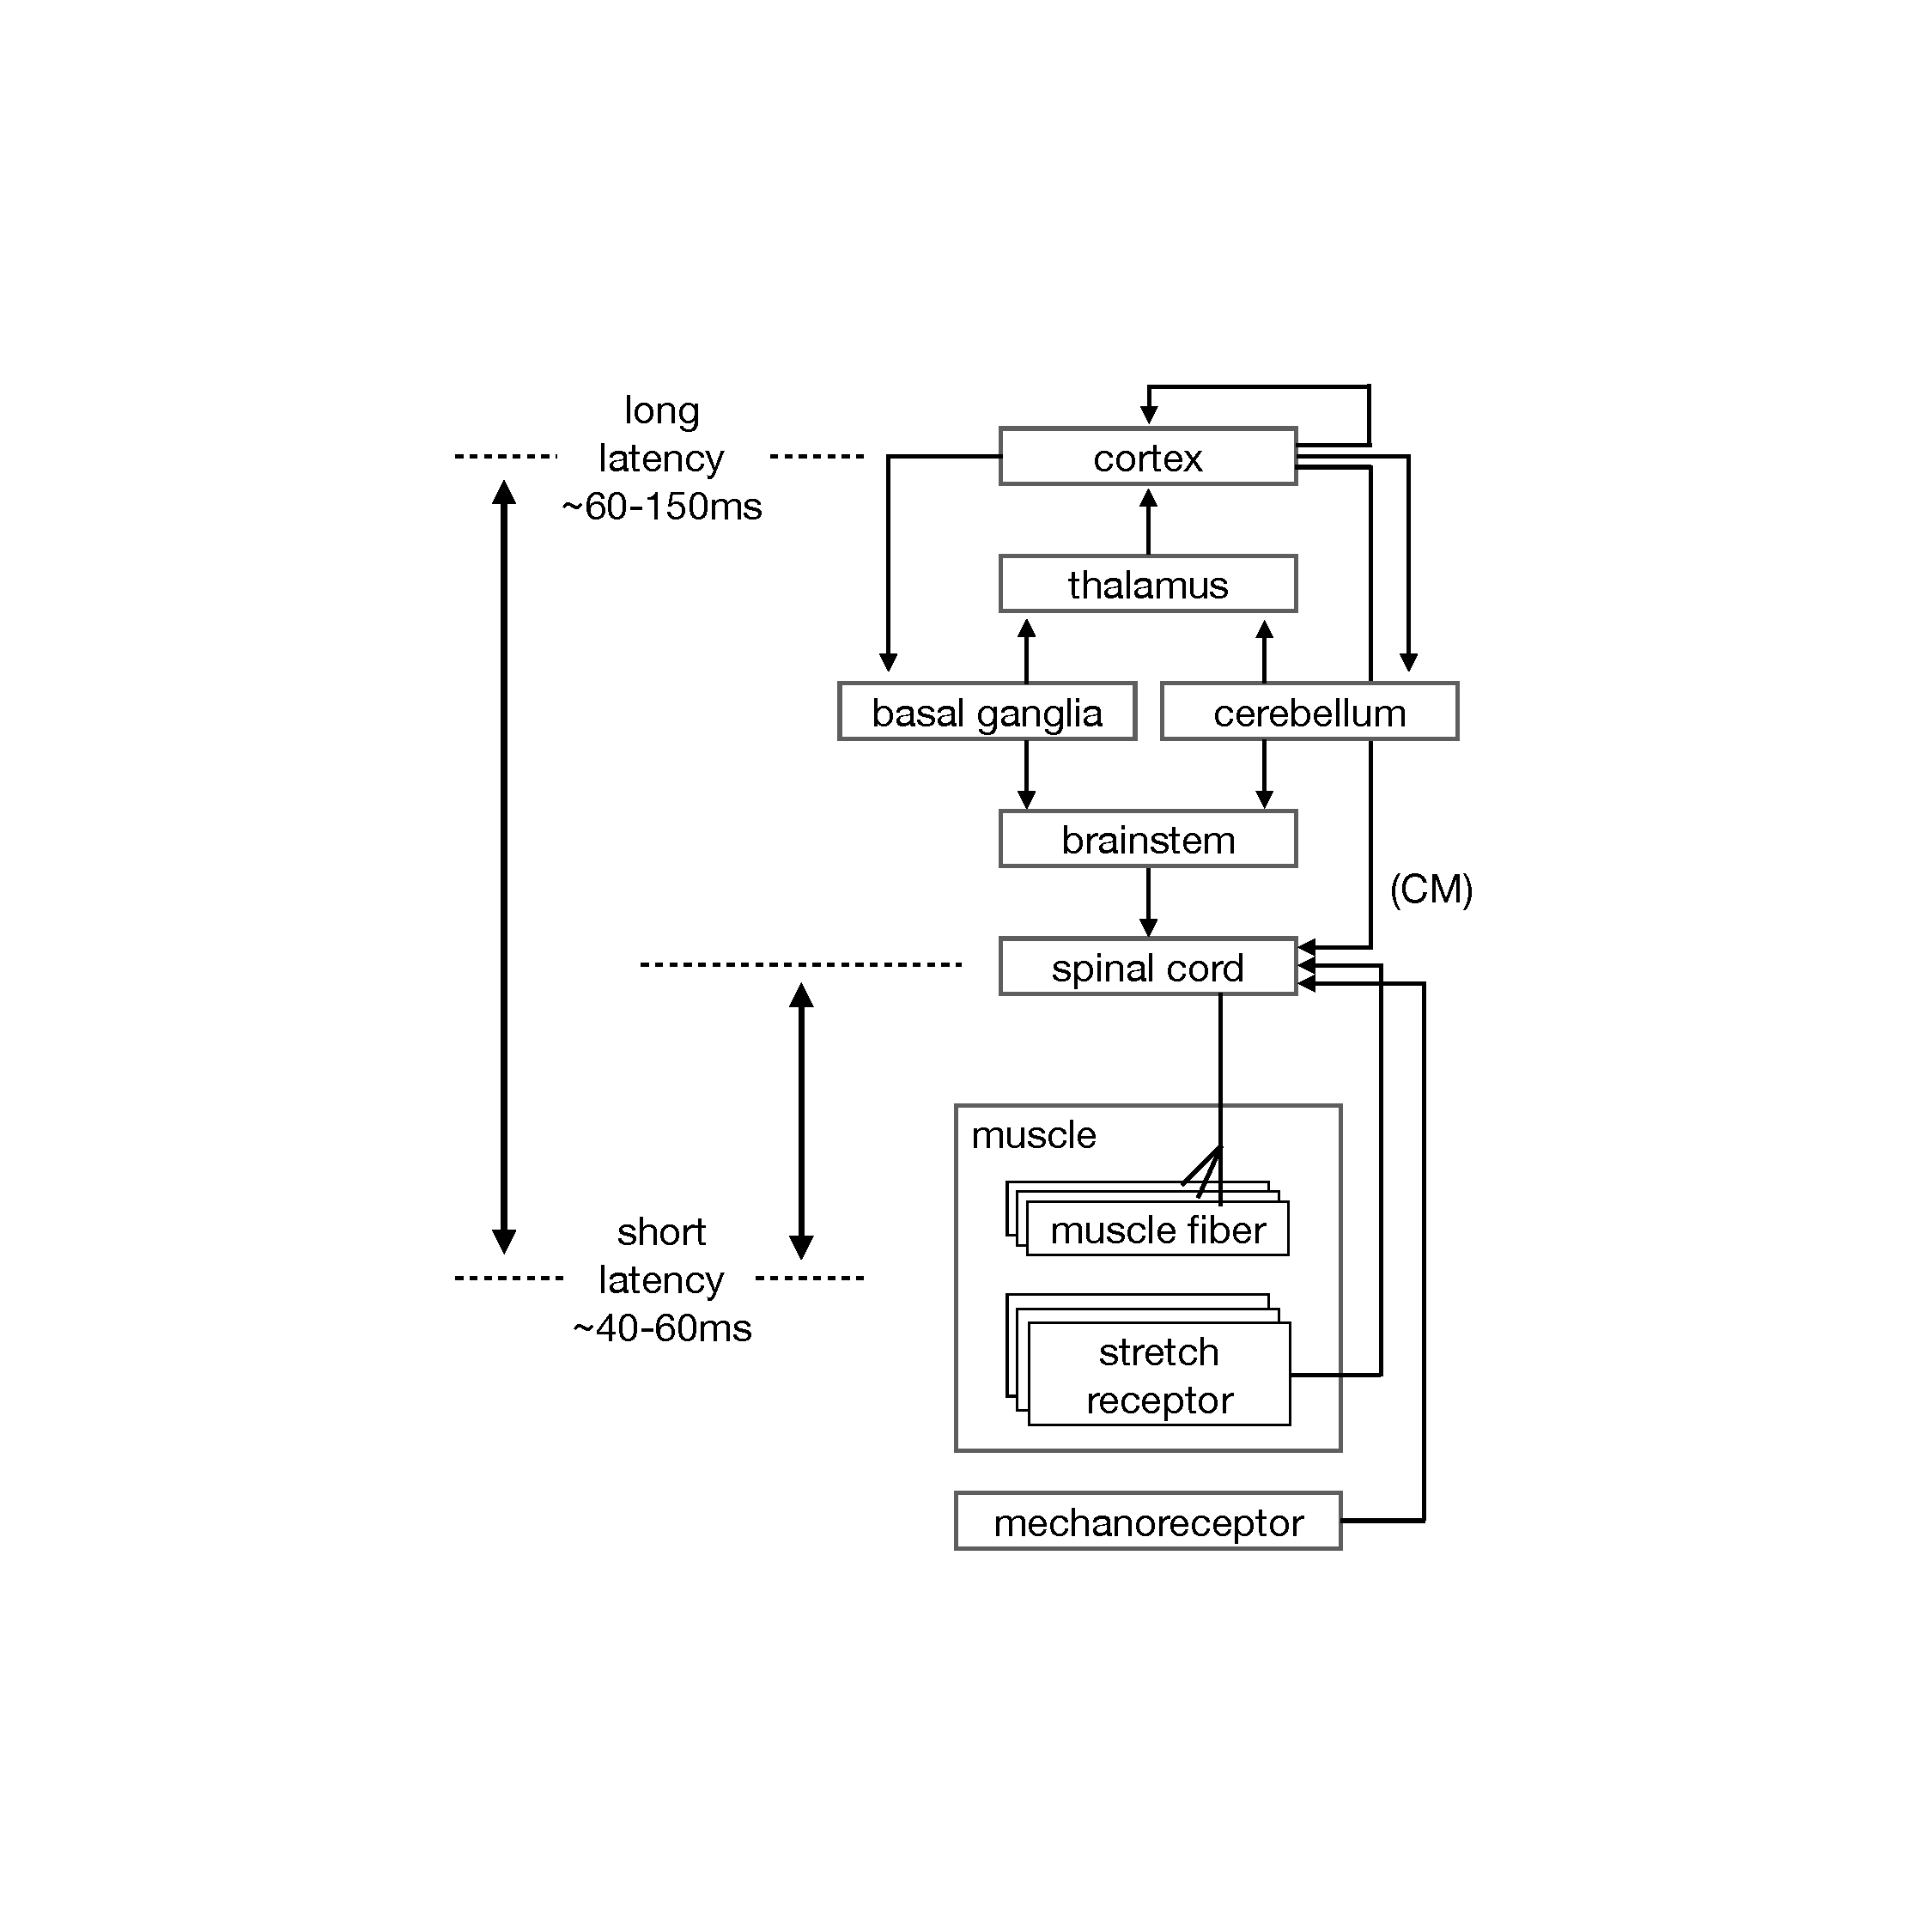
\includegraphics[width=1.0\textwidth]{background_theory/motor_system.pdf}
\caption[Motor sytem schematic]{Overview sketch of the motor system depicting the the redundancy of the system both hierarchically (multiple muscle fibers are innervated by the same motor neuron, many motor neurons innervate the same muscle) as well as heterarchically (parallel spinal, corticomotoneuronal, cerebellum, basal gangliar feedback loops). Parallel reflex responses can be classified as long latency (approximately 60-150ms) and short latency (approximately 60ms). We hope to consider the parallelism and redundancy of the motor system to inspire our data analyses and models of motor computation.}\label{fig:motor_system}
\end{figure}





\section{EMG Studies of Motor Learning}

There are several notable studies which leveraged electromyography (or similar interfaces) in the context of motor learning. We provide a brief comparison between these studies to illustrate where this work fits into the context of the field.

Mosier et al.\cite{MosierRemappingHandMovements2005} used a human-machine interface glove, capturing angles of the finger joints, to characterize how subjects learned to remap hand movements in an isometric force task. They found that subjects could readily adapt to dramatically altered mappings, that subject variability in both the input and output space decreases over learning, and that subjects preferred rectlinear task solutions, straight line movements, to targets. This study provides an excellent foundation for developing decoders from a high-dimensional input space into a 2-dimensional task space. We used this study as an inspiration in task design, trading joint angles for direct readouts of muscle activity.

In Radhakrishnan et al. (2008)\cite{radhakrishnanLearningNovelMyoelectricControlled2008,Mussa-IvaldiSensoryMotorRemapping2011}, the authors developed a task in which subjects controlled a 2-dimensional cursor using abstract myoelectric mappings. This study found that subjects could readily learn non-intuitive motor contingencies, and tracked the modulations of muscle tuning functions over learning. By applying perturbations, namely vibration to increase proprioceptive noise, the study interpreted subjects' abilities to maintain learning despite this noise as a sign that subjects were internalizing a model of the decoder. They found that subjects were able to learn ``novel synergies'', which we view as support for synergies as a solution to a redundant motor task as opposed to a constraint. These studies suffer from the fact that the number of degrees of freedom is much lower than that which the movement system leverages in natural tasks. We attempt here to increase the dimensionality of our task to provide a more naturalistic learning environment.

Valero-Cuevas and colleagues\cite{Valero-Cuevas2009} used intramuscular EMG to track muscle activation patterns of all muscles driving a single fingers during a force production task. They found that, due to the redundancy between the motor input (7 muscles) and the output (3 force directions), subjects tended to ``accumulate'' variability in the task-irrelevant null space, as this activity did not penalize subjects on the task. However, this experimental design did not track learning of a new task, rather control over a finger in a reasonably naturalistic movement scenario.

De Rugy et al.\cite{derugyMuscleCoordinationHabitual2012} and Berger et al.\cite{BergerDifferencesInAdaptationRates2013a} examined changes in muscle synergies and coordination patterns when subjects' EMG mappings are altered in various ways (removing a muscle, rotating the mapping out of a subject's synergy-space). Their analyses revealed preferential use of arm vs hand muscle groupings depending on the task constraints, pointing to the advantage of greater ability to fractionate distal muscles. This is supported by the myoelectric study by Dyson et al.\cite{Dyson2018} which showed that intrinsic hand muscles showed greater ability to control a decoder task compared to forearm muscles. The ``suboptimal'' responses by subjects in De Rugy and Berger's tasks suggest the lack of use of an internal model for this type of adaptation on the timescales of the studies. This suggestion is one we pursue further in this study.

More recently, researchers at CTRL-Labs have explored using wrist- and hand-based dynamic, mobile myoelectric interfaces as a generic, non-invasive neural control interface for human-machine interaction\cite{ctrl-labsatrealitylabsGenericNoninvasiveNeuromotor2024}.

Overall, myoelectric studies face key limitations. Firstly, EMG signals are inherently noisy and can be affected by factors like cross-talk from adjacent muscles. Extracting reliable measures of muscle coordination is non-trivial. That said, there is an incredible about of signal within EMG data, thus despite significant crosstalk complex decoding can supply a high-bandwidth interface to probe learning. Secondly, It remains unclear if the brain explicitly optimizes a high-dimensional control policy, or if learning involves differential selection and adaptation of lower-dimensional muscle coordination patterns. As discussed, our view is the latter, and we believe that EMG interfaces such as the one used here, clarify that coordination patterns emerge as solutions by a neural controller, rather than fundamental constraints ``baked into'' the system.


% % existing models of learning?

% Models of Adaptation
% - two-rate models \cite{smithInteractingAdaptiveProcesses2006}
% - linear dynamical system for adaptation \cite{chengModelingSensorimotorLearning}

% - Optimal feedback control, now introduced to motor control field 25 years ago, remains the best (most elegant) explanation we have for motor coordination, but there's no adaptation or learning.
% - Optimal feedback control as an algorithm which generate minimally intervening motor actions

% kenneth craik first suggested internal models \cite{craikNatureExplanation1967}

% % Forward model -- predictive -- from action to future state (system ID)
% % Inverse model -- kinematic/kinetic transformation from future state to action (control "law")
% % Error between these models drives learning?

% The control setup writes a cost, environment has some dynamics.

% expanded into broader field of RL... 

% - A policy is a function of your ``state'' where the output is motor actions, decisions about which muscles to activate. Policies can be formalized as a probability distribution over actions, and can be parameterized in a number of ways, from simple distributions to dynamical systems, to neural networks.



\section{Internal Models and Motor Learning}

The prominent theoretical framework for understanding motor control and learning relies on the concept of internal models in the brain. Proposed at the very beginning of modern neuroscience, an internal model is a neural representation, or function, which captures the input-output properties of the motor system and environment\cite{craikNatureExplanation1967}. Two key forms of internal models have been proposed:

\begin{itemize}
    \item \textbf{Forward Models} which predict future sensory consequences given the current state and motor commands. Learning forward models is essentially a system identification problem, mapping actions to their impacts on future states to build predictive capacity.
    \item \textbf{Inverse Models} which generate the motor commands required to achieve a desired future state given the system's current state. Inverse models do just that: they \textit{invert} the intended state to generate the necessary motor actions.
\end{itemize}

The discrepancies between the outputs of these two internal models are hypothesized to drive motor learning: errors between the predicted and actual sensory feedback from executing a motor command can be used to update forward and inverse models over time. Optimal feedback control theory provided an early and elegant explanation for motor coordination\cite{todorovOptimalFeedbackControl2002}. However, it did not incorporate adaptation or learning mechanisms. More recent theoretical efforts have expanded on internal models and their role in motor learning within the broader field of reinforcement learning. In this view, a policy maps the current state to a distribution over possible motor actions or muscle activations. Policies can take various parametric forms, from simple distributions to dynamical systems or neural networks.

Several specific hypotheses have been proposed regarding how the brain acquires and adapts internal models and policies. Some posit hierarchical processes with two-rate models, where a faster adaptive process updates an existing skill while a slower process gradually learns a new skill from scratch \cite{smithInteractingAdaptiveProcesses2006}. Linear dynamical system models have also been used to descriptively model sensorimotor adaptation\cite{chengModelingSensorimotorLearning}.

Internal models set the stage for the key question: what computations are the brain performing during motor learning? Two competing hypotheses have emerged:
%
\begin{itemize}
  \item \textbf{Model-Based Learning}: This view aligns with internal model theories, positing that the brain builds and refines explicit representations to solve motor problems, in the manner of optimal control. While providing an elegant computational foundation, pure model-based learning is computationally intensive, especially when learning models of highly complex dynamical systems like the musculoskeletal system.
  \item \textbf{Model-Free Learning}: An alternative is that we rely on learned memories of state-action mappings and their associated rewards acquired through trial-and-error interaction with the world. Model-free methods are efficient for simple tasks, but can face challenges in higher dimensions and when attempting to generalize across tasks. 
\end{itemize}
%
In reality, the brain may leverage a combination of both model-based and model-free strategies. It has been proposed that the brain constructs \emph{approximate} internal models as a focusing mechanism to constrain model-free learning\cite{dawModelBasedInfluencesHumans2011}. While internal models provide a powerful conceptual framework and have been tested extensively across a variety of tasks which positive results, there remains limited direct evidence of their neural implementation. Computational models can capture behavior, but bridging the gap to localize explicit neural representations of these models has proven challenging. It remains unclear if the brain encodes distinct inverse and forward models, or constructs more integrated representations. Additionally, while internal models are motivated by principles of optimal control, human motor learning often appears not to conform to true optimality, instead displaying systematic biases and inconsistencies \cite{loebHierarchicalFoundationModels1999,loebHardLessonsMotor1987}.





\section{Discussion}

Based on the research reviewed above, it is clear that the neural control of the hand is composed of a number of complex, overlapping, massively redundant control schemes. These ``controllers'' receive goal information as well as contextual and perceptual information pertaining to the ongoing task; they contain all available task context and branch downstream to an array of spinal centers and individual innervations to produce rewarding movements.

That is, the movement system is highly distributed throughout the brain and body, constructing actions based on a variety of state dependencies\cite{sejnowskiPerspectivesCognitiveNeuroscience1988}. The physiology reveals this distributed nature, constructing and adapting actions based on feedback by constantly selecting, composing, and adapting control policies to make motor decisions.

We hypothesize that subjects will utilize this vast repertoire of pre-existing control schemes, movements, controllers, patterns, and activations to find patterns which increase task success. They will then ``hone'' this scheme by refining the discovered movement pattern. This predicts an initial exploratory or ``search'' period in the task, followed by (or overlapping with) an exploitative period as subjects settle on a motor solution.


% Certain movement disorders may involve information bottlenecks in communicating the policy given the current state~\cite{gershmanRewardcomplexityTradeoffSchizophrenia2020}. Optimal compression requires knowing state probabilities, implying some form of internal model -- the marginal state distribution or mean state occupancies. The memory demand of policies can act as an information bottleneck in action selection~\cite{pirayLinearReinforcementLearning2019}. A ``default policy'' may represent habits. We speculate that practice and expertise involve convincing the brain to commit to a more complex policy or maintain commitment at the current level of complexity.

% Ultimately, a key challenge for researchers is to identify the cost functions subjects employ and the learning rules used to update their policies during motor learning.


\cleardoublepage\printendnotes%
\ifSubfilesClassLoaded{%
    \newpage%
    \bibliography{../bib/bibliography}%
}{}%
\end{document}
